\documentclass{scrartcl}
\usepackage{tikz}
\usepackage{amsmath}
\usepackage{amssymb}
\usepackage{unicode-math}
\setmathfont{Asana Math}

\newcommand{\selection}{\sigma}
\newcommand{\projection}{\pi}
\newcommand{\rename}{\rho}
\newcommand{\join}{\Join}
% \fullouterjoin defined by unicode-math
\newcommand{\semijoin}{\ltimes}
\newcommand{\groupby}{\Gamma}

\newcommand{\mtt}[1]{\text{\texttt{#1}}}

\setlength{\parindent}{0pt}

\begin{document}

\section*{Exercise 1}

Canonical translation:

\begin{center}
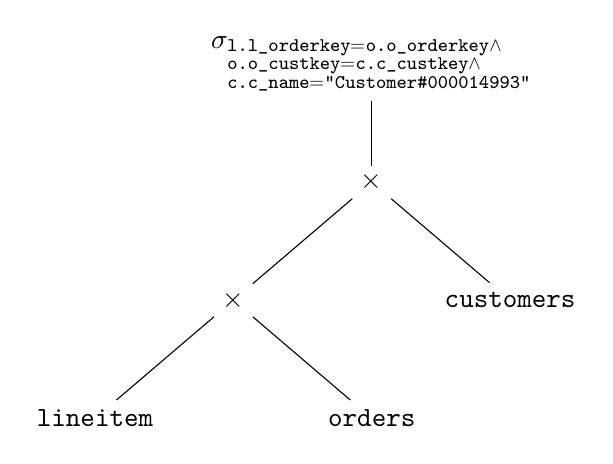
\begin{tikzpicture}[sibling distance=10em]
    \node {
        $\selection_{\begin{subarray}{l}
                        \mtt{l.l\_orderkey} = \mtt{o.o\_orderkey} \wedge \\
                        \mtt{o.o\_custkey} = \mtt{c.c\_custkey} \wedge \\
                        \mtt{c.c\_name} = \mtt{"Customer\#000014993"}
                     \end{subarray}}$
    }
    child {
        node {$\times$}
        child {
            node {$\times$}
            child {node {\texttt{lineitem}}}
            child {node {\texttt{orders}}}
        }
        child {node {\texttt{customers}}}
    };
\end{tikzpicture}
\end{center}

Logical optimization:

\begin{center}
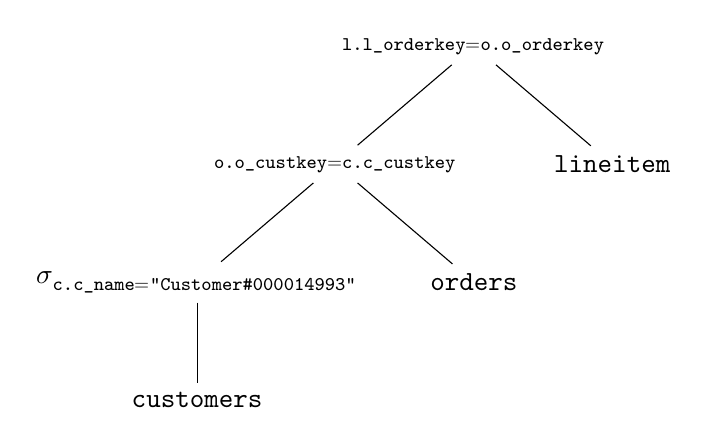
\begin{tikzpicture}[sibling distance=10em]
    \node {$\join_{\mtt{l.l\_orderkey} = \mtt{o.o\_orderkey}}$}
    child {
        node {$\join_{\mtt{o.o\_custkey} = \mtt{c.c\_custkey}}$}
        child {
            node {$\selection_{\mtt{c.c\_name} = \mtt{"Customer\#000014993"}}$}
            child {node {\texttt{customers}}}
        }
        child {node {\texttt{orders}}}
    }
    child {node {\texttt{lineitem}}};
\end{tikzpicture}
\end{center}

\subsection*{Exercise 2}

\subsubsection*{1.}

If we know that $R1.x$ is a key, we know that a given value for $x$ can only
occur at most once. So we can estimate the selectivity by $\frac{1}{|R1|}$.

\subsubsection*{2.}

If we know that both $R1.x$ and $R2.y$ are keys, every tuple will be joined with
at most one other, so the output size is limited to $\min\{|R1|, |R2|\}$. This
means we can estimate the selectivity by $\frac{\min\{|R1|, |R2|\}}{|R1| \cdot
|R2|}$.

If we know that only $R1.x$ is a key, the argument still holds: Every tuple from
$R2$ will only be joined with at most one tuple from $R1$. So we can estimate
the selectivity by $\frac{|R2|}{|R1| \cdot |R2|}$.

Analogously, if only $R2.y$ is a key, we can estimate the selectivity by
$\frac{|R1|}{|R1| \cdot |R2|}$.


\subsection*{Exercise 3}
\subsubsection*{NL}
For running over the left side we need 10000ms for transferring the pages to the core (I/O transfer rate). Furthermore,
we need 10ms for the first page to seek (random access cost). All other pages are assumed to lie next on disk, hence we
ignore the seek costs. Summing all up we get for each run through the right side costs of 10010ms.
Since we have 1000 * 50 tuples on the left side we get the total cost for the right side with 1000 * 50 * 10010ms.
Additionally accessing the left side we need to seek 1000 pages, since all right side pages are in between those might
not be in RAM anymore. Also we have (1/10000)s transfer cost. Hence, we need additional 1000 * 10.1ms.
\begin{align}
1000 * 10.1 ms + 1000 * 50 * 10010ms = 500510100 ms
\end{align}


\subsubsection*{BNL}
For running over the left side we need 10000ms for transferring the pages to the core (I/O transfer rate). Furthermore,
we need 10ms for the first page to seek (random access cost). All other pages are assumed to lie next on disk, hence we
ignore the seek costs. Summing all up we get for each run through the right side costs of 10010ms.
Since we can compare 100 pages at the same time on the left side we get the total cost for the right side with
(100/1000) * 10010ms. Additionally accessing the left side we need to seek (100/1000) pages, since all right side pages
are in between those might not be in RAM anymore. Also we have (100/10000)s transfer cost.
Hence, we need additional (100/1000) * 20ms.
\begin{align}
100 * 20 ms + 10 * 10010ms = 102100 ms
\end{align}

\end{document}
